\section{Mate pair sequencing}

\textbf{The mate pair sequencing is basically a variation of the classic
sequencing with pair-end reads} (see section about NGS).

In both cases the reading of the filament starts from opposite directions 
and two reads are produced. The central sequence of the insert remains unknown,
even if we know the size (\textit{inner mate distance}).

The main difference lies in the fact that in the mate pair sequencing the DNA
fragment is first circularized and then broken again.

\subsection{Steps for the construction of a mate pair library}

The DNA is fragmented as usual. Subsequently are selected, among those larger
(typically comprised from 2 to 20 kb) fragments of a certain length, determined
a priori (for example 2kb).

So here we proceed to the \textbf{circularization} of the DNA fragments,
usually after the addition of a biotinylated probe (sonda) to each of the two
ends.

The DNA is circularized and then fragmented again. 

At this point, we proceed to the selection of the fragments containing
the biotinylated probes, which are formed by the joint end of the
original fragment.

The addition of the biotinylated probes allowes the identification of the ends
without having to carry out the alignment.

Then adapters and primers are added in each end of the biotinylated
fragment. The sequencing starts from those two ends and goes in opposite
directions.

Finally we obtain the reads of the two ends of the original
fragment, just as in a sequencing with pair-end reads.

To better understand the described steps you can take a look at the figure
\ref{fig:mate_pair}.

\begin{figure}[H]
  \centering
  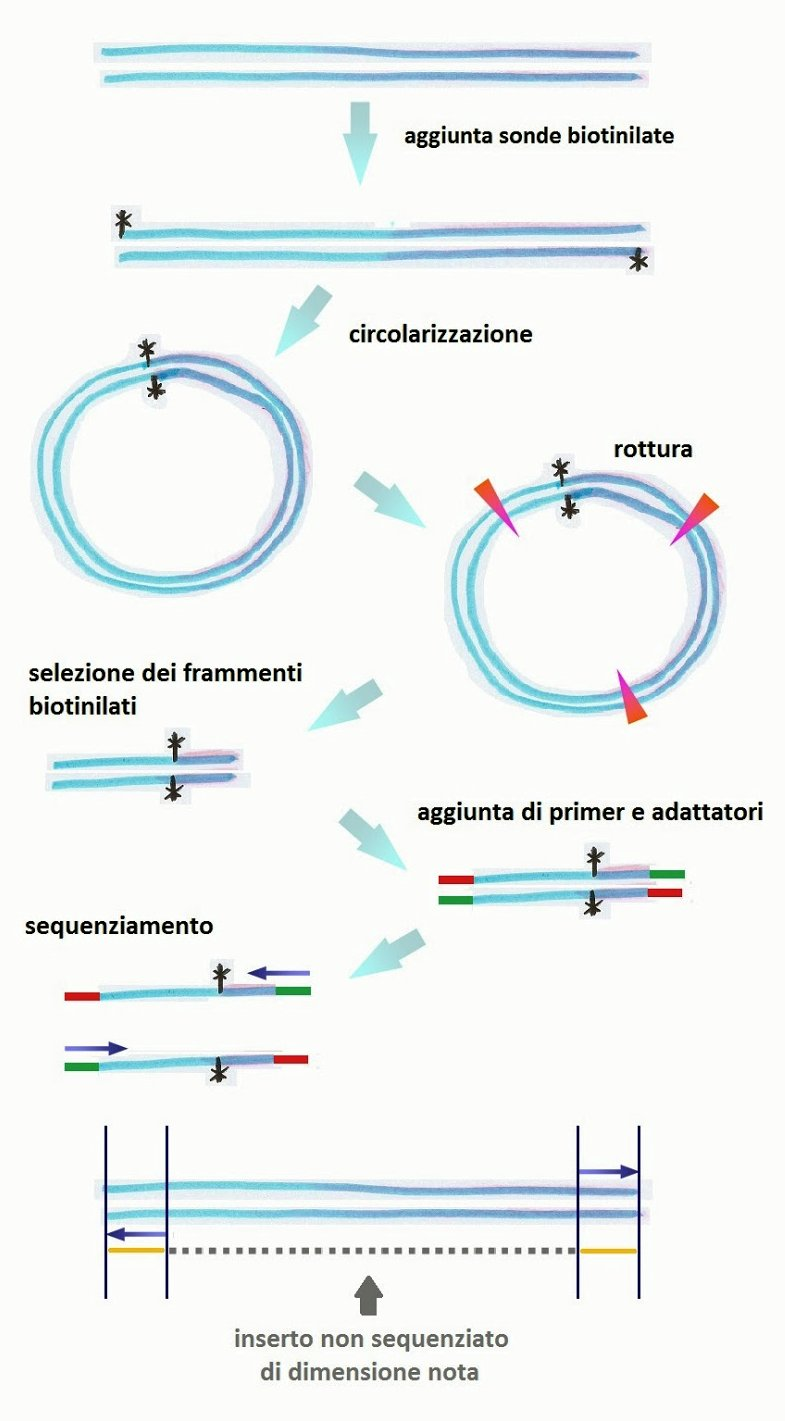
\includegraphics[scale=0.3]{mate_pair}
  \caption{mate pair sequencing}
  \label{fig:mate_pair}
\end{figure}

\paragraph*{How can mate pair sequencing identify rearrangements?}

Very simple: suppose you have a mate pair library originally constructed
with fragments of 2kb, and a system for the production of reads 200 bases each.

So we know from the start that the inner mate distance must necessarily be
equal to $2000 - 200 = 1600 bp$.

If in the process of alignment with the reference genome sequences the reads
of a patient are separated by 1600 bp, it means that the patient does not have
insertions or deletions.
If the reads mapped at different distances (more or less), the patient will
have a rearrangement (a deletion or an addition respectively).

\section{Mate paired libraries}

There are two types of coverage: sequence coverage and physical coverage.

The pair-end aren't the same as mate-pairs.
Pair-end reads can be easily obtained from the library clone: firstly the 
sequence from one end is obtained, then with the other primer we can obtain the 
sequence from the other end.

\paragraph*{Problem with NGS sequencing} The chemistry for library 
amplification does not permit to manage fragments of DNA longer than a few 
hundred bases.
\paragraph*{Mate pair libraries overcome the limits of paired end libraries}
The trick is to do a circular DNA. At the end of this process you have a
library with million of this pairs, and this help enormously the assembly of
the genome.

\section{Detection of structural variation with mate pair libraries}

How can we estimate where there is a structural variation? We can plot the 
structural forms and see if there are some point that aren't in the normal 
distribution. Mate pairs can also be useful to discover structural variation in 
a genome as compared to a reference genome.
